\chapter{X-Ray Absorption Fine-Structure Spectroscopy}
\label{chapter: XAFS}

The method of X-ray Absorption Fine-Structure Spectroscopy (XAFS) probes the electronic structure of atoms in a material by 
irradiating a sample with X-rays and recording the resulting absorption spectrum. As this diagnostic technique constitutes the purpose of the spectrometers designed in this work, it will be elaborated on in the following.

XAFS originates from X-ray Absorption Spectroscopy (XAS), a method 
first experimentally established in 1918-1920 at Lund University in a series of experiments by K. Stenström and H. Fricke under the supervision of M. Siegbahn \citep{siegbahn1925spectroscopy, mottana2013}. Although XAS was 
overshadowed by X-ray Diffraction (XRD) in its first few decades, in large part due 
to the higher x-ray intensity requirements, it had a key advantage in that it 
could probe less ordered and liquid materials. As such, the technique 
experienced a boom in 1975, where the building of 
large research facilities with electron synchrotrons enabled consistent 
access 
to intense x-ray sources \citep{stumm1989history}. This also 
marks the advent of XAFS, the modern version of XAS, allowing measurement of 
the fine structures of absorption edges, which presents the opportunity to 
locally probe defects and features in lattice 
structures to a 
higher degree than other x-ray diagnostics. With 
over 50\% of beamtime requests from industrial customers for synchrotron 
laboratories pertaining to x-ray absorption methods, XAFS has become a 
well-established tool to evaluate samples for a wide array of fields, 
including 
Chemistry, Biology and Material Science 
\citep{mottana2015historical}.

XAFS is not only limited to conventional samples, but can also be applied to probe short-lived, dynamic states such as WDM \citep{eason1984improved}, which exists in a non-crystalline state where 
short-range order dominates, making XAFS especially suited as a diagnostic 
technique \citep{levy2009x}. X-ray sources 
capable of short pulses, like laser-produced plasma, or spectrometers using detectors 
with 
rapid recording, like image plates or CCD cameras, enable the collection of a complete spectra on the order of nanoseconds. The first experiment using XAFS on WDM was conducted in in 
1987, 
in which converging laser-induced shocks were used to bring an aluminum 
sample 
to WDM conditions \citep{hall1988experimental}. Since then, XAFS has been 
widely used in WDM matter research, with x-ray crystal spectrometers playing 
a 
central role \citep{riley2021warm, levy2009x, torchio2016probing}.

In the 
context of WDM 
experiments, XAFS often examines the photon energy 
range 
around a 
K-edge, defined by the binding energy of K-shell 
electrons in a material. By studying the fine-structures of 
the absorption spectra in this region, multiple properties of WDM, e.g. density, 
temperature, and coordination of atoms, can be 
simultaneously extracted \citep{levy2010double, 
torchio2016probing, hall1988experimental}. These 
structures 
consist of shifts in the location and 
shape of the K-edge, as well as oscillations in the 
absorption coefficent after the edge, and originate from free electrons ejected by x-rays 
through the photoelectric effect. In a simplified 
description as depicted in fig \ref{XAFS_scheme}, the wave-functions of the ejected electrons scatter on neighboring atoms, so that a 
part of the free electron wave-function returns to 
and interferes with the absorbing atom. As this all 
occurs in a single coherent quantum state, the 
process is effectively a modulation 
of the quantum electronic state at the location of 
the absorbing atom. Since the absorption coefficient 
depends on the available electronic states, this 
phenomenon causes modulation of the absorption 
probability, and therefore the absorption 
spectrum, depending on the atomic order within 
$\approx 5\angstrom$ of the absorbing atom 
\citep{newville2014fundamentals}. 

\begin{figure}
	\centering
	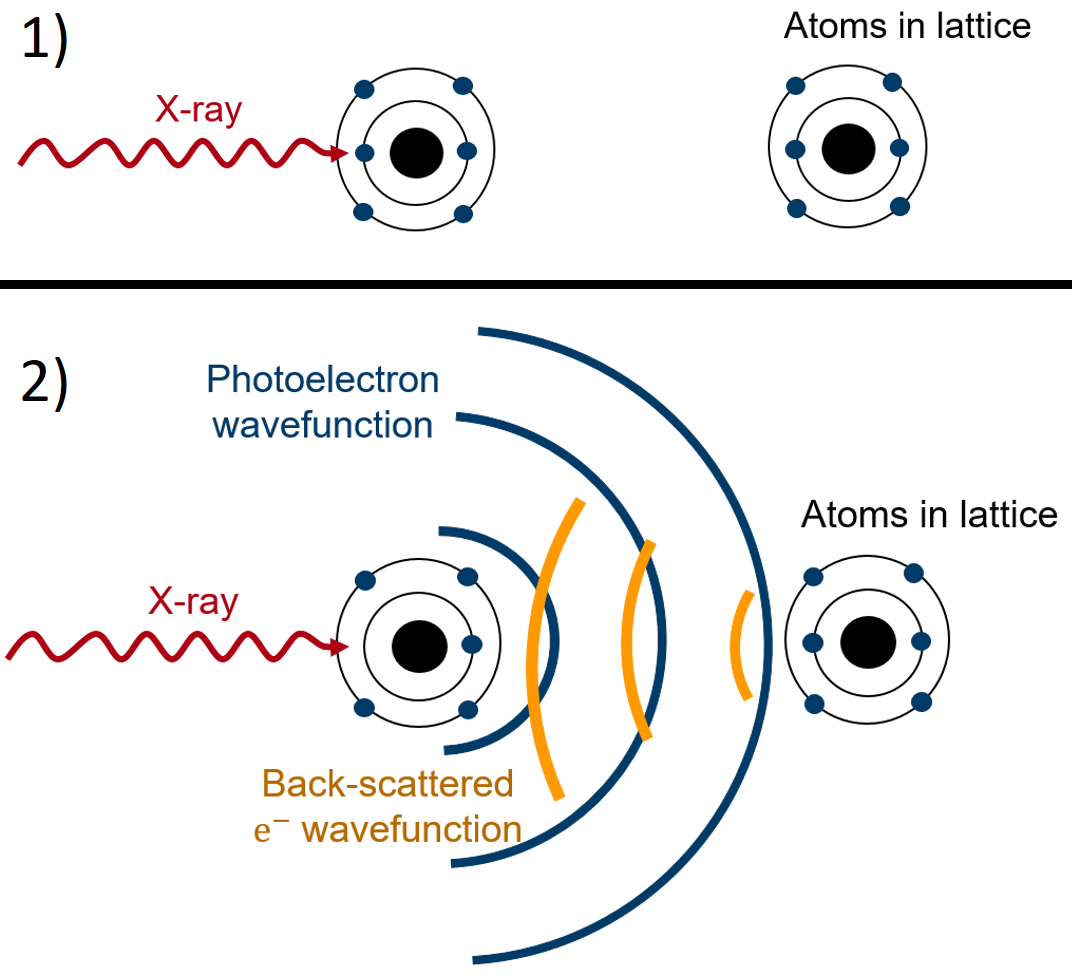
\includegraphics[width = 0.55\textwidth]{Diagrams/XAFS_scheme.PNG}
	\caption{Schematic representation of XAFS mechanism. 1) An electron is 
	ejected from the absorbing atom through the photoelectric effect. 2) The 
	electron wavefunction is partially back-scattered by a neighboring atom 
	in a lattice, which returns to the absorbing atom and modulates the 
	electronic states, consequently modulating the absorption coefficient.}
	\label{XAFS_scheme}
\end{figure}

XAFS can be broken 
down into two techniques: X-ray Absorption Near Edge 
Structure (XANES), covering the range of 
\SI{50}{\electronvolt} within the K-edge 
\citep{peyrusse2009k}, and Extended X-ray Absorption 
Fine-Structure (EXAFS), extending as far as \eV{250} 
above the edge \citep{fontaine1979soft}. In the case 
of XANES, 
the shift and slope of the K-edge are governed by the 
degeneracy, ionization, and continuum lowering of the 
plasma and are affected by the electronic temperature and 
density  \citep{falk2018experimental, levy2009x}. For EXAFS, the amplitude of the absorption 
oscillations is an indicator of ionic temperature, while 
the 
position and frequency of the peaks reveal 
information about the density and ionic order 
\cite{riley2021warm}. Note that determining 
properties from the oscillations is more 
straightforward for EXAFS, as approximations of 
single scattering are valid in this region, 
simplifying theoretical models 
\citep{newville2014fundamentals}.

To give an idea of what XAFS absorption spectra typically look like and 
how WDM properties can be determined from them, I will summarize two 
experiments, with one applying XANES and the other EXAFS, whose results are 
depicted in fig. 
\ref{XAFS_examples}. In an experiment conducted by Levy\textit{ et al.} 
\citep{levy2009x} corresponding 
to fig. \ref{XAFS_examples}a, WDM of aluminum is produced through isochoric 
heating with a picosecond proton beam pulse generated by Target Normal Sheath 
Acceleration (TNSA) on gold targets. The sample is then irradiated with x-rays 
from a laser-driven plasma backlighter of erbium, allowing for recording of 
absorption spectra. By fitting theoretical models and simulations to the 
experimental near-edge curves, WDM quantities can be extracted. For example, the electron 
temperature is determined through the variable slope of the K-edge, where a 
steeper slope indicates a lower temperature. Likewise, the electron temperature 
can be found by studying the far-edge structures, as shown in fig. 
\ref{XAFS_examples}b. In this experiment by Torchio \textit{et al.} 
\citep{torchio2016probing}, iron samples are compressed and brought to WDM 
conditions through laser-driven shocks, then diagnosed with x-rays from a synchrotron beamline specialized for x-ray absorption 
techniques. The electron temperature is determined through comparison of the experimental EXAFS to theoretical models. In addition, information about the atomic structure of the sample 
is gained by studying the disappearance of certain peaks. Notable is also the 
decreasing amplitude of EXAFS oscillations with increasing temperature, which is 
indicative of a collapse of atomic order in the material. 

\begin{figure} [H]
	\centering
	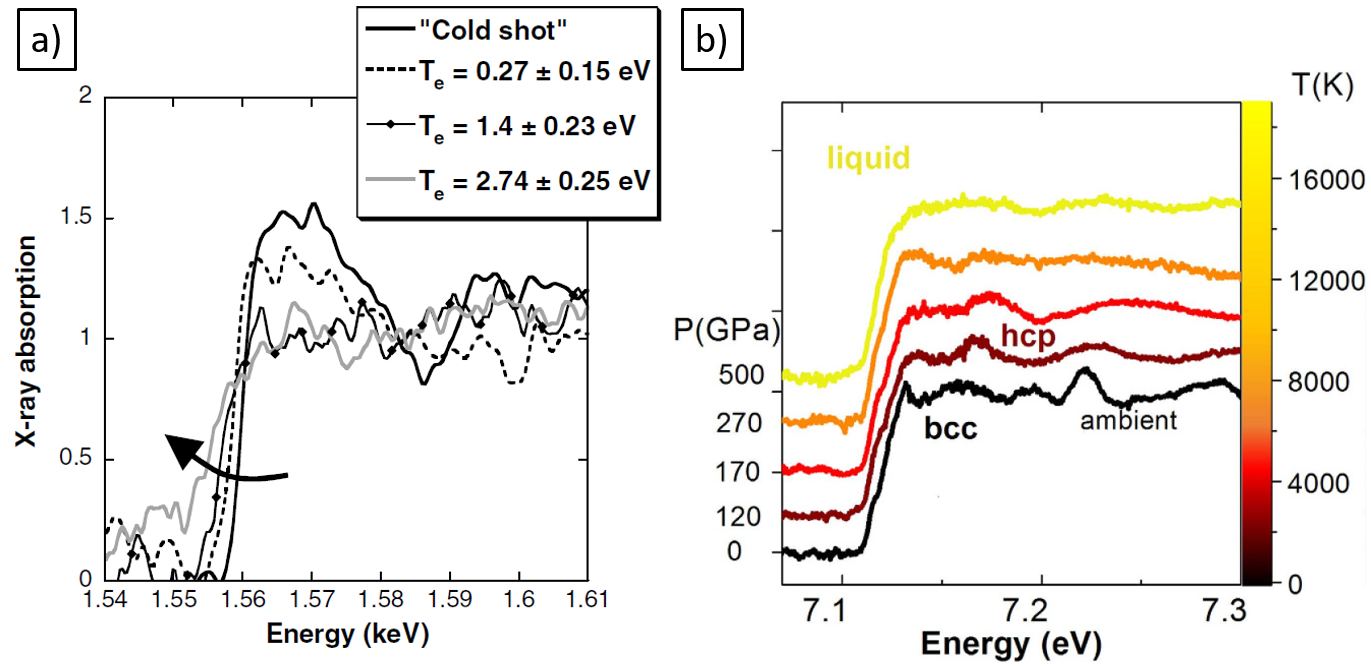
\includegraphics[width = \textwidth]{Diagrams/XAFS_examples.PNG}
	\caption{Examples of XAFS spectra taken in WDM experiments for XANES and 
	EXAFS respectively. It is important to note that the first graph displays 
	absorption spectra of aluminum, while the second shows spectra of iron. 
	\textbf{a)} Spectra from an aluminum sample isochorically heated to WDM 
	conditions with energetic proton beam and diagnosed with x-rays from 
	laser-driven plasma of erbium. XANES is applied to extract information 
	about the electron temperature \citep{levy2009x}. 
	The arrow highlights the reduction of the K-edge slope with rising 
	temperature.
	\textbf{b)} Spectra from an iron sample brought to WDM conditions with a 
	laser-driven shock and investigated with x-rays generated by a synchrotron. 
	EXAFS is conducted to derive the temperature and lattice structure of the 
	samples. Note that the spectra are artificially shifted along the y-axis to 
	represent rising pressure \citep{torchio2016probing}.}
	\label{XAFS_examples}
\end{figure}

Both of these results exemplify the power of XAFS as a diagnostic method for 
warm dense matter. As with most experiments in this vein, this method is made 
possible by x-ray spectrometers. Due to a number of restrictions originating 
from inherent properties of these devices and the volatile nature of WDM, the design of these spectrometers is essential for experimental success. As such, I will 
go into more depth on their history and design in the following chapter. 